\documentclass{article}
\usepackage[utf8]{inputenc}
\usepackage{cite}
\usepackage{graphicx}
%\usepackage{mathtools}
\usepackage{amsmath}
%\usepackage{mathptmx}
%\usepackage{amsfonts}
%\usepackage{amssymb}
\usepackage{url}
\usepackage{color}

%\renewcommand*\rmdefault{dayroms}
\setlength\parindent{0pt} % Geen /newline gezeik ;)
%\renewcommand{\familydefault}{\ttdefault}
\renewcommand*\sfdefault{cmss}
\newcommand{\horrule}[1]{\rule{\linewidth}{#1}}
\title{	
	\normalfont \normalsize
	\horrule{2pt} \\[0.25cm]
	\huge Hardware Security: JavaCard \\
	\large Design document - petrol allowance \\
	\large Radboud University Nijmegen\\
	\horrule{0.5pt} \\[0.125cm]
}
\author{\normalsize \textbf{Group 2:} Wouter Kuhnen (s4081420), Wouter van Kranenburg (s4319176),\\\normalsize Ye Myat Kaung (s4460677),  Stephanie Silvius (s4380479)}

\date{\today}

\begin{document}


\maketitle
\newpage
% Chapters
% !TeX root = main.tex

\section{Introduction}
\label{introduction}
This design document is written for the course Hardware Security for the petrol allowance case and will describe the use cases, assets and stakeholders, security requirements, threats and abuse cases, attacker model and will include a high level design of the system. 
 % Introduction
% !TeX root = main.tex

\section{Use cases}
The use cases we have defined are:
\begin{itemize}

\item Personalisation of the petrol card with the issuer terminal (IT):\\
During the personalisation phase the petrol card will have to be initialised with key material, a card identification number and the current petrol balance will be set to zero. This will be done by the card issuer with their issuer terminal. The petrol card will also have to be registered to a car owner and a check needs to be in place to see if the car owner didn't already receive a petrol card, however this is out of the scope of this document.

\item Charging the petrol card at the charging terminal (CT): \\
Each month the charging terminal will receive a petrol allowance update. This update determines the petrol allowance that will be written to all petrol cards. Once a petrol card presents itself, the charging terminal will have to validate if the petrol card is still valid, if it is the card owner will have to enter a PIN to authenticate himself to the terminal. The card owner can then choose to either view his current balance or charge the monthly petrol allowance to his petrol card balance. Writing petrol allowances to petrol card balances will not be possible once, sub-charges during the month will not be possible. The new petrol balance on the petrol card will be immediately available for getting petrol. 

\item Getting petrol at the petrol terminal (PT):\\
At the petrol terminal the card owner is able to get petrol. He presents his petrol card to the PT, where he can see his current petrol allowance, after choosing the type of petrol, the PT will remove the current petrol balance from the petrol card by writing a balance of zero. After the transaction has been completed the updated balance will be written back to the petrol card. 

\item End-of-life: \\
Once a card reaches end-of-life (EOL), it has to be blocked and possibly decomissioned. 

\item Stolen Card: \\
If a card gets stolen, the identification number of the card and all it's key material will have to be blocked and revoked. During the night, all petrol and charging terminals will be updated with a list of blocked petrol cards. After 5 years, the petrol card will automatically be blocked.

\end{itemize} % Usecases
\section{Assets}
Our project case involves the following assets:
\begin{itemize}
\item Petrol

\item Smartcards
\begin{itemize}
 \item Current allowance on the card
 \item Card identification number
 \item PIN code
 \item Timestamp indicating last charge
 \item Public and private key created during personalisation
 \item Certificate from CA
 \item Signed timestamp of last checked revocation list by CA
 \item List of revoked certificates
\end{itemize}

 \item Charging terminals
 \begin{itemize}
 	\item Current monthly allowance to be charged to cards
 	\item List of blocked cards
 	\item Public and private key created during personalisation
 	\item Signed timestamp of last checked revocation list by CA
  	\item Certificate from CA
	\item List of revoked certificates
 \end{itemize}

 
 \item Petrol terminals
 \begin{itemize}
  	\item Certificate from CA
 	\item List of blocked cards
 	\item Public and private key created during personalisation
 	\item Signed timestamp of last checked revocation list by CA
 	\item List of revoked certificates
 \end{itemize}

 
 \item Personalization terminals
 \begin{itemize}
	\item Certificate from CA
	\item Public and private key created for secure communication
 \end{itemize}

 
 \item Back-end
 \begin{itemize}
 	\item Public and private key
 	\item List of revoked certificates
 	\item List of ID numbers associated with each terminal and cards
 \end{itemize}

\end{itemize}
 % Assets
\section{Stakeholders}
We have identified the following stakeholders as being relevant for the project:
\begin{itemize}
\item Car owners. These are the users of the systems and the holder of the smartcards.
They will typically want easy usable systems and a certain degree of privacy. 
Some of them may try to bypass the system to get more fuel than allowed.

\item Local petrol station owners. They will have to modify their pumping installations to 
work with terminals. They typically want low costs and low interaction for maintenance.

\item Petrol companies with multiple pumping stations. They will have to modify their
pumping installations to work with terminals. They typically want low costs and 
low interaction. When possible, they might attempt to track customers via their smartcard.

\item The government. They are the ones who want this system in place, to be able to regulate
the fuel consumption. They typically want the system to be secure and fair.
\end{itemize}

 % Stakeholders
\section*{Assumptions}
During the design of the project, several assumptions were made, they are listed here.
\begin{itemize}
\item Smartcards
\begin{itemize}
	\item A car owner can only have one petrol card
	\item The smartcard is tamper-resistant, therefore provide integrity and confidentiality of their data and functionality
\end{itemize}

\item Charging
\begin{itemize}
\item Terminals come preinstalled which is done securely
\item MITM attacks are possible
\end{itemize}


\item Pumping
\begin{itemize}
\item The pump is not rigged; will always communicate the right amount of fuel that has been released to the terminal 
\item Terminals come preinstalled which is done securely
\item MITM attacks are possible
\end{itemize}

 
\item Personalization
\begin{itemize}
\item Employees personalising smartcards will not be able to steal key material.
\item Employees who created the back-end did not have malicious intentions, such as building a backdoor
\end{itemize}

\item Back-end
\begin{itemize}
\item Maintains a list of blocked card IDs
\end{itemize}
\end{itemize}

  % Assumptions
\section{Attacker model}
At any point in time it is likely that an attacker will perform a MiTM or a card tear. The compromise of a key material on the card should not bring down the entire petrol system. The attackers will not be able to tamper with the petrol cards, nor will they be able to build a backdoor in the software of the terminals.

We will now broadly define $3$ categories of attackers, although overlap may occur. For example research may fall into the hands of criminals. 

\begin{itemize}

\item (Organised) criminals

This groups capabilities will include organised crime such as extortion and violence to obtain legitimately issued petrol cards. On the other hand it will also include card owners who may intentionally try to game the system by removing the petrol card from the terminal during a transaction. This group will mostly try to obtain more petrol than rationed.

\item Insiders

Members of this group will have some sort of access to the inner workings of the system. This includes configuration of any of the terminals the system uses within the limits allowed by the software. It also includes the designers of the system, who are not to be trusted with the master key. This group may try to bring down or sabotage the workings of the system for a larger group of users.

\item Researchers
This group is sometimes provided with full specification on a system or it's protocols. They are likely to break protocols such that they can intercept and manipulate any traffic between the petrol card and a terminal. This group will typically include researchers at an university, which gives an indication of the amount of time and money available. The goal of this group will be to break the security model in any way worthy of a publication.
 
\end{itemize} %Attacker model

\section{Security requirements}
% --- Start of the entire list ---
\begin{enumerate}
% --- Start of Confidentiality ---
\item Confidentiality
	\begin{enumerate}
	\item The card identity number shall only be revealed to the  personalisation/charging/pump terminal after the terminal has been authenticated to the petrol card.
	\item The public key material shall only be revealed to the personalisation/charging/pump terminal after the terminal has been authenticated.
	\item The card usage shall not be revealed to any kind of terminal.
	\item The PIN code shall only be know by the petrol card and the petrol card owner. 
	\item The monthly petrol allowance update shall only be revealed after the terminal has been authenticated to the back-end. 
	\end{enumerate}
% --- End of Confidentiality ---
%\begin{minipage}{\linewidth}
% --- Start of Integrity ---
\item Integrity
	\begin{enumerate}
	\item The petrol allowance on the petrol card can only be altered by an authenticated terminal.
	\item The identity number of the petrol card cannot be altered. 
	\item The public and private keys of the petrol card cannot be altered.
	\item The logs on the terminal can only be altered by the terminal itself. 
	\end{enumerate}
% --- End of Integrity ---
%\end{minipage}

% --- Start of Authentication ---
\item Authentication during charging
		\begin{enumerate}
		\item The petrol card shall authenticate to the charging terminal by using its public and private key% its identity number (IDnr).
		\item The charging terminal shall authenticate itself to the petrol card  by using its public and private key.
		\item The charging terminal shall authenticate itself to the back-end with the public and private key to receive the monthly petrol allowance that can be written to the petrol cards.
		\end{enumerate}	
		
\item Authentication during pumping
	\begin{enumerate}
	\item The petrol card shall authenticate to the pumping terminal by using its public and private key. % providing its identity number (IDnr).
	\item The pumping terminal shall authenticate itself to the petrol card by using its public and private keys
	\item The pumping terminal shall authenticate itself to the back-end by using its public and private keys.
	\item The card owner shall authenticate to the pumping terminal and petrol card of its ownership by providing the PIN to the petrol card.
	\end{enumerate}		
% --- End of Authentication ---


% --- Start of Availability ---
\item Availability
	\begin{enumerate}
	\item \textcolor{red}{The car-owner should still be able to use the pumping terminal even if the pump terminal has no connection to the back-end.}
	\end{enumerate}	
% --- End of Availability ---


% --- Start of Authorisation ---
\item Authorisation
	\begin{enumerate}
	\item The charging terminal is only authorised to update the petrol allowance on the petrol card once every month.
	\item The pumping terminal is authorised to withdraw the petrol allowance during petrol pumping from the petrol card.
	\end{enumerate}
% --- End of Authorisation ---


% --- Start of Non-repudiation ---
\item Non-repudiation
	\begin{enumerate}
%		\item The petrol card shall obtain proof that the allowance value came from the back-end via the charging terminal.
%		\item The petrol card shall obtain proof that the changed allowance value came from the pumping terminal.
		\item The charging terminal can prove to the back-end that it charged the monthly allowance to a valid petrol card. 
		\item The pump terminal can prove to the back-end that it collected petrol allowance from a valid petrol card.
	\end{enumerate}
% --- End of Non-repudiation ---

\end{enumerate}
% --- End of the entire list ---
	%Security Requirements
\section*{Design decisions}
During the design of the project, several design decisions were made, they are listed here.
\begin{itemize}
\item Smartcards
\begin{itemize}
\item PIN Code is used for authenticating the card owner to the terminals.
\item Public Key Infrastructure is used here to secure communication with terminals.
\item The card comes to the user, already personalized, but not charged
\item All communication between smartcard and terminal is encrypted, except for the first communication of the certificate by either one party.
\end{itemize}

\item Charging terminal
\begin{itemize}
\item Charging terminal cannot sign allowance itself but communicates the allowance that has been signed by the backend.
\item All communication between backend and terminal is encrypted, except for the first communication of the certificate by either one party.
\item Charging can only be done once a month and only the whole allowance in one time. Allowance cannot be charged in parts.
\item The charging terminal can see the allowance stored on the smartcard.
\end{itemize}

\item Petrol terminal
\begin{itemize}
\item Will ask for amount of fuel that is to be released. Card holder knows how much fuel is going to be used. Once entered, the card holder does not get rest of allowance back. So the pump terminal is not able to write allowance to the card.
\end{itemize}

\item Personalization
\begin{itemize}
\item We assume this is done in a secure way, so this is out of the scope of the 
implementation.
\end{itemize}

 
\item Back-end
\begin{itemize}
	\item Will have a signed list of blocked cards that are issued to the terminals.
	\item Will have a list of all the ID numbers associated with each card and terminal in the petrol allowance eco-system.
	\item Will have the utmost level in the certificate chain apart from the main CA.
\end{itemize}
\end{itemize}
	% Design decisions
\section{Overall design}
\subsection{PIN codes}
The user will have to enter a PIN code on the terminal numpad to verify ownership of the petrolcard to the terminal. The terminal will send this PIN + signed by its private key to the smartcard. By which the smartcard will reply with whether the PIN number is correct or not.

\subsection{Cryptography}
A certificate consisting of a public and private key will be first created on the back-end (the overall system acting as the Certificate Authority). Whenever a new smartcard is personalized, it will store the certificate of the CA, create public and private key for itself and a time-stamp of the last update of certificate revocation list which is signed by the CA certificate. Each terminal will have the same setup: CA certificate, its own public and private key, and signed time-stamp of last updated certificate revocation list.

\subsection{CA certificate stored in Terminals/Smartcards}
The main certificate from the CA stored in each terminal and smartcard is used to verify the validity and authenticity each certificate during communication. Each end point, i.e both smartcard and terminal alike, will verify the certificate of the other end point it is connecting to, whether the certificate has been revoked or not by the CA. This way when the CA has been notified of abuse or breach in one of the end points, it will only take 24 hours for each end point to know of the revocation of a particular certificate.

\subsection{Public and Private key in Terminals/Smartcards}
Public and private keys in each end point will be used in conjunction with the CA certificate to mutually authenticate between each other. It is also used to negotiate a symmetric key and also to provide integrity of the message by signing them.

\subsection{Life Cycle of Card}
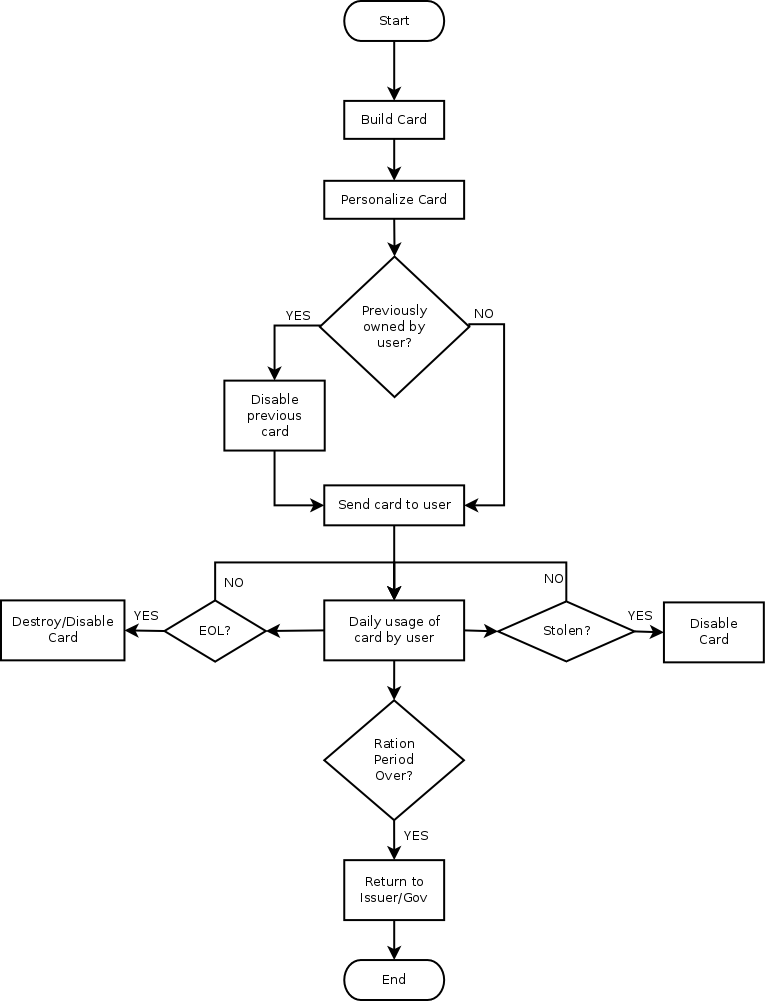
\includegraphics[width=\textwidth]{SCLifeCycle}

\subsection{Protocol Descriptions}

\subsubsection{Terminology}
	\begin{tabular}{*{2}{l}}
	 $ENC\{X\}$ & encryption function for X with symmetric key agreed to by both parties:\\
	 $SIG\{X\}_{privkey}$ & signing function for X with private key of sender. \\
	 $certificate_{T}$ & certificate of Terminal \\
	 $pub_{T}$ & public key of Terminal \\
 	 $priv_{T}$ & private key of Terminal  \\
	 $IDnr_{T}$ & Identification (ID) number of Terminal \\
	 $Nonce_{T}$ & Nonce from Terminal \\
	 $SK$ & Symmetric Key \\
	 $Verify$ & Certificate Verification function \\
	 $H$ & Cryptographic Hash function \\
	 $Slog$ & Secure Logging function \\
	 $T$ & Terminal (charging/petrol) \\
	 $JC$ & JavaCard (smartcard) \\
	 $BE$ & Back-end (most closet communication to CA)\\
	 $CVR$ & Certificate Validity Request \\
	 $PIN$ & PIN number \\
	 $PIN_{AUTH}$ & True or False response based on in-/valid PIN \\
	 $C_{pt}$ & current possessed petrol points (in liters) \\
	 $A_{pt}$ & current monthly petrol allowance (in liters) \\
	 $W_{pt}$ & wanted petrol points (in liters) \\

	\end{tabular} 
	
\subsubsection{Mutual Authentication}
T $\to$ JC: commandAPDU to enable applet.\\
T $\to$ JC: $certificate_{T}, pub_{T}$\\
JC: $Verify(certificate_{T})$ and choose SK\\
JC $\to$ T: $ENC\{SIG\{IDnr_{JC}\}, certificate_{JC}\},  [ENC]_{pub_T}$\\
T $\to$: $Verify(certificate_{JC})$\\
T $\to$ JC: $SK\{[H(IDnr_{T}||Nonce_{T})]_{priv_T}+IDnr_{T}+Nonce_{T}\}$

% %$SK\{[H(IDnr_{S}||Nonce_{S})]_{priv_S}$ where S is senderG$

\subsubsection{Certificate Validity Request}
Note: this is considered to be done via a secure communication after mutually authenticating between smartcard $\to$ terminal, terminal $\to$ backend and smartcard $\to$ backend through terminal.
\\
\\
JC $\to$ BE: $[CVR + pub_{JC}]_{pub_BE}$\\
BE $\to$ JC: $[H(validity||TS||Certs)_{priv_BE}+validity+TS+Certs]_{pub_JC}$\\

\subsubsection{PIN validation and authorisation}
Note: this is considered to be done via a secure communication after mutually authenticating each other.
\\
\\
T $\to$ JC: $SK\{[H(PIN||Nonce_{T})]_{priv_T}+PIN+Nonce_{T}\}$\\
JC $\to$ T: $SK\{[H(PIN_{AUTH}||Nonce_{JC})]_{priv_JC}+PIN_{AUTH}+Nonce_{JC}\}$\\

\subsubsection{Petrol usage}
Note: this is considered to be done via a secure communication after mutually authenticating each other.
\\
\\
JC $\to$ T: $SK\{[H(A_{pt}||C_{pt}||Nonce_{JC})]_{priv_JC}+A_{pt}+C_{pt}+Nonce_{JC}\}$\\
T $\to$ JC: $SK\{[H(W_{pt}||C_{pt}||Nonce_{T})]_{priv_T}+W_{pt}+C_{pt}+Nonce_{T}\}$\\
JC: $Slog([H(IDnr_{T}||W_{pt}||C_{pt})]_{priv_T}+IDnr_{T}+W_{pt}+C_{pt})$\\
T: $Slog([H(IDnr_{JC}||W_{pt}||C_{pt})]_{priv_JC}+IDnr_{JC}+W_{pt}+C_{pt})$\\
 %Overall design
%\input{organisation}\newpage
%\input{reflection}

%{} sym
%[] pub
\end{document}
